%! TEX root = ../main.tex
\documentclass[main]{subfiles}

\begin{document}

\chapter{GNSS品質監視に基づく自己位置推定}
\label{ch:method}

本章では,農業用ハウスのようにGNSSの品質が不安定な環境においても,
ロバストに動作する自己位置推定システムを構築する.
具体的には,LIOとRTK-GNSSを統合し,電波の遮蔽やマルチパスによる誤差を抑制する手法について述べる.
なお,本章ではRTK補正を前提とした出力をRTK-GNSS,それらを総称してGNSS観測と呼ぶ.

本手法の特徴は,受信機の状態量に基づく判定と,LIOの移動量との整合性を利用したGNSS品質監視モジュールを提案する点にある.
このモジュールは,見かけ上の精度情報が良好であっても,
実際にはマルチパスなどの影響で数メートルの誤差が含まれる観測値をリアルタイムで検知し,棄却する.
提案手法によって,バックエンドのグラフ最適化に信頼できるデータのみを選別して投入することで,
長時間走行における自己位置推定の安定性を向上させる.

\section{システム構成}
\label{sec:system_overview}
本研究で構築した移動ロボットシステムは,
農業用ハウスにおいて自己位置推定と環境センシングを同時に行うことを目的として設計されている.
本システムは,周囲の環境とロボットの状態を観測するハードウェア系と,
それらの情報を統合して位置推定およびマッピングを行うソフトウェア系で構成される.
システム全体の構成とデータの流れをFig.~\ref{fig:system_overview}に示す.
以下では,ハードウェア,ソフトウェア,および各座標系の関係について述べる.

\begin{figure}[t]
  \centering
  \includegraphics[width=0.9\linewidth]{figures/3/system.png}
  \caption{Overview of the system architecture and data flow. 
          The PC-side ROS 2 runs RTAB-Map to generate a 
          globally consistent map and pose estimates, while the AGV-side ROS 2 
          runs FAST-LIO2 to provide registered point clouds and odometry. 
          Sensor topics are exchanged via ROS 2.
          Navigation2, incorporating STVL for 3D obstacle avoidance, 
          serves as the decision-making layer. It processes the SLAM 
          data to generate and send velocity commands to the AGV.}
  \label{fig:system_overview}
\end{figure}

農業環境では,電波の遮蔽やマルチパスによりGNSSの品質が大きく変動する.
また,ハウス内通路のような単純な形状の場所では,
LiDARによる推定が不安定になる縮退が発生しやすい.
これらの環境特性を踏まえ,本研究では観測データの品質変動を考慮した統合手法を採用する.

以下では,まず移動ロボットの車体と搭載センサについて述べ,
次にLIO,ナビゲーション,およびGNSS品質監視に基づくソフトウェア構成について説明する.

\subsection{移動ロボットプラットフォームと搭載センサ}
\label{subsec:hardware}
移動ロボットには,不整地走行に適したAGV車体を用い,
圃場内を巡回しながらセンサデータを取得できる構成とした.
車体にはGmade社のGS02を採用した.
環境認識と自己位置推定のために,3D-LiDAR(Livox Mid-360)を使用する.
LiDAR点群は地図生成と自己位置推定に使用する.また,LiDAR内蔵のIMUは,
点群の歪み補正や短時間の姿勢推定に利用する.Livox Mid-360 の外観と仕様を付録\ref{appendix:Livox-MID360}に示す.

絶対位置の計測には,RTK-GNSS受信機(u-blox ZED-F9P)を用いる.
基準局からの補正データ(森林総合研究所のRTK基準局サービス\cite{jforest_rtk}を利用)を
無線LAN経由で取得し,屋外環境においてセンチメータ級の精度を目指す.
ZED-F9P受信機およびアンテナの外観と仕様を付録\ref{appendix:ZED-F9P}\ref{appendix:ANN-MB-00}に示す.


一方で,ハウス周辺では作物や構造物の影響で,測位状態が不安定になることが確認されている.
そのため,本研究ではGNSSデータを常に信頼するのではなく,
品質監視に基づいて自己位置推定への重み付けを動的に制御する.

ロボットの駆動にはBLDCモータを使用するが,
不整地でのスリップを考慮し,車輪オドメトリは自己位置推定としては用いない.
センサデータの取得と処理はRaspberry Pi 4Bで行い,
無線LANを介してPCと通信を行う.AGVの外観と構成をFig.~\ref{fig:robot_platform}に示す.

\begin{figure}[t]
  \centering
  \includegraphics[width=\linewidth]{figures/3/AGV.pdf}
  \caption{Overview of the AGV and onboard sensors used in this study.}
  \label{fig:robot_platform}
\end{figure}

\subsection{ソフトウェア構成}
\label{subsec:software}
本システムはROS~2(Robot Operating System 2)\cite{ref:ROS2} を基盤とし,
自己位置推定と地図生成をモジュール化して構成している.
具体的には,フロントエンドにLIOを用いることで高頻度な位置推定を行い,
バックエンドではRTAB-Map\cite{ref:2018rtabmap}によってループ閉じ込みや因子グラフ最適化を実行する.
さらに,提案するGNSS品質監視モジュールによって選別・調整されたRTK-GNSSデータを,
バックエンドの位置制約として統合する仕組みとした.

また,将来的な自動走行への対応を確認するため,
Navigation2\cite{ref:Navigation2}を接続している.
これにより,生成された地図や座標系TFが標準的なナビゲーションシステムでそのまま利用可能であることを確認した.
なお,本研究の主な評価対象は自己位置推定の精度と地図の整合性であり,
自動走行性能自体の定量評価は本論文の範囲外とする.

\subsubsection{ROS~2}
\label{subsubsec:ros2}
ソフトウェア基盤にはROS~2を採用する.
ROS~2はDDSに基づく通信機構を備え,分散処理,実運用における信頼性,およびモジュール再利用性の観点から,
研究開発用ロボットシステムの構築に適している.本研究では,各センサのデータ取得,自己位置推定,地図生成,
および自動走行をノードとして分離し,トピックおよびTFにより統合する.

\subsubsection{Navigation2}
\label{subsubsec:navigation}
自動走行アプリケーションとしてROS~2のNavigation2(Nav2)を用いる.
Nav2は,グローバル経路計画(Global Planner),ローカルプランニング/追従制御(Local Controller),
およびBehavior Treeによるタスク実行を統合的に提供するナビゲーションフレームワークである.
本システムでは,RTAB-Mapが提供する\texttt{map}座標系での自己位置推定結果に基づいて経路計画を行い,
出力された速度指令を\texttt{cmd\_vel}として車体へ送信する構成とした.
また,局所障害物の表現にはSpatio-Temporal Voxel Layer(STVL)\cite{ref:stvl}を用い,
3D LiDAR点群をボクセルとして保持することで局所コストマップを生成する.
加えて,研究室内の静的環境において,経路生成から\texttt{cmd\_vel}出力までの
基本動作を確認した(Fig.~\ref{fig:nav2_indoor_appendix}).
ただし,本研究では室内での基本動作確認に留まり,
農業用ハウス環境における自動走行性能の定量評価は未実施である.

\subsubsection{LiDAR--IMUオドメトリおよびSLAM}
\label{subsubsec:lio_slam}
フロントエンドにはFAST-LIO2\cite{ref:fast_lio2}を採用し,
LiDAR点群とIMU計測から高頻度の相対オドメトリを推定する.
FAST-LIO2は,高速なスキャンマッチングとIMU統合により,
リアルタイムでの安定した動作が可能である.

バックエンドにはRTAB-Mapを用い,ループ閉じ込みと因子グラフ最適化によって地図の整合性を向上させる.
採用の理由は,まずループ閉じ込みによる長期的なドリフト抑制すること,
次に複数のセンサ情報を制約として統合できる枠組みを備えていることが挙げられる.
さらに,将来的にカメラなどのセンサを追加する場合でも拡張が容易であり,
農業環境でのマッピングへの発展性が高い点である.

\subsubsection{座標系とTF構成}
\label{subsubsec:tf}
本システムの座標系は,ROS 2の構成に従って設計されている.
FAST-LIO2はオドメトリ(\texttt{odom} $\rightarrow$ \texttt{base\_link})を推定し,
RTAB-Mapは地図との整合性を保つための全体的な補正(\texttt{map} $\rightarrow$ \texttt{odom})を担う.
また,車両中心(\texttt{base\_link})からLiDARやアンテナへの位置関係は,
静的なパラメータとして定義している.

\subsubsection{データ処理フロー}
\label{subsubsec:dataflow}
システムの情報の流れは以下の通りである.
まず,FAST-LIO2が点群とIMUデータからロボットの相対的な移動量を計算する.
同時に,GNSS品質監視モジュールが受信機のGNSS状態とLIOの移動量を比較し,
信頼できるGNSSデータのみを選別・調整する.次に,RTAB-Mapがこれらの情報と点群を統合して地図を作成し,
ループ閉じ込みによる軌跡の最適化を行う.この地図と自己位置をもとに,
Navigation2が経路計画と走行制御を行う.最終的に,最適化された軌跡に環境センサの値を対応付けることで,生育環境マップが生成される.

\clearpage
\section{農業用ハウス環境におけるGNSS観測異常の分類}
\label{sec:problem_definition}
農業用ハウス環境において,RTK-GNSSは一時的に精度が低下することがある.
これは,ハウスの骨組みや作物による電波の遮蔽,反射,あるいは補正情報の中断などが原因である.
本研究では,これらの品質低下のGNSS信号を区別すべき3つの故障モードとして整理する.

第一に,GNSS利用不可である.これは,電波の遮蔽や補正データの途絶により,
測位解そのものが得られない,あるいは情報として使えない状態を指す.

第二に,NLOSやマルチパスによる大きな誤差である.
これは,受信機の表示が良好で誤差の推定値も小さいにもかかわらず,
実際には位置が数メートル飛んでしまう状態である.
本研究では,この見かけ上は正しいが実際には誤っているデータを排除することに注目する.

第三に,LIOの縮退である.ハウスの通路など形状が単純な場所では,
LiDARのデータだけでは位置を特定しにくくなり,縮退が発生しやすい.
また,不整地では車輪がスリップしやすいため,車輪オドメトリは位置推定には適さないと判断した.

本研究の目的は,GNSSが不安定な環境において,誤ったデータをグラフ最適化に含めないことを最優先としつつ,
精度の高いRTKデータを用いてLIOの累積誤差を抑えるシステムを構築することである.
そのために,バックエンドに送るデータを選別する品質監視モジュールを設計する.

\clearpage
\section{提案手法:GNSS品質監視モジュールの設計}
\label{sec:supervisor}
本研究の最優先課題は,RTAB-Mapに入力されるGNSSデータによって地図の精度が低下するのを防ぐことである.
そのため,GNSSデータをリアルタイムで選別する品質監視モジュールを設計した.
農業用ハウスでは,電波の遮蔽や反射,補正情報の中断により,大きな誤差が含まれる可能性がある.
このとき,誤ったデータが1つでもRTAB-Mapに入力されると,
地図全体が歪んでしまう.したがって,本手法ではGNSSの重みを調整するのではなく,採択または遮断の二値制御を適用する.

\subsection{入出力仕様と遮断の実装}
\label{subsec:supervisor_io}
品質監視モジュールには,GNSSの観測値,
受信機の状態量,およびLIOが出力する移動量を入力する.
モジュールは,入力されたGNSSデータを以下のどちらかで出力する.

\begin{itemize}
  \item 採用: データをそのままRTAB-Mapへ送り,本来の共分散を保持する.
  \item 遮断: 観測値を無効と見なし,バックエンドへの転送を停止する.
  共分散行列の対角成分を極大値に置き換えることで,そのデータを実質的に無効化する.
\end{itemize}
反射波などの影響がある環境では,受信機が精度は良いと誤判定して小さな共分散を報告することがある.
この場合,単に重みを少し軽くするだけでは誤ったデータの影響が残ってしまう.
そこで本研究では,遮断時には共分散を固定の大きな値(例:$99999$)に設定し,
$$\mathrm{diag}(C_{\mathrm{blk}},C_{\mathrm{blk}},C_{\mathrm{blk}})$$
として拘束を確実に無効化する実装とした.

\subsection{可用性判定}
\label{subsec:availability_gate}
可用性判定は,受信機自身が出力する情報に基づき,
データの基本的な妥当性を確認する.その目的は,測位の失敗や補正データの中断など,
明らかに利用不可能な状態のデータを事前に遮断することである.

具体的には,測位モードや衛星数などの情報をトリガとして遮断を行う.
ただし,受信機の情報が一時的に遅延することもあるため,
情報が取得できないからといって直ちに遮断するのではなく,
明確なエラー条件を満たした場合のみ遮断する.

また,起動直後はデータの履歴が足りず,
後述する整合性検定が正しく動作しないことがある.
そのため,開始直後の一定期間は初期化区間とし,
可用性判定のみで妥当性を確認してデータを通すようにした.
これにより,システム起動直後にデータが連続して遮断されるのを防いでいる.

\subsection{完全性監視:短時間増分整合性検定}
\label{subsec:integrity_gate}
完全性監視は,受信機の状態が良好であっても,
NLOSなどによって生じる大きな位置誤差を検知するための仕組みである.
本手法では,絶対位置を直接比較するのではなく,
短い時間($\Delta T$)の間にロボットが微小時間$\Delta T$におけるLIOの相対変位とGNSSの相対変位の整合性を評価する.

時刻$t$におけるGNSSの位置を$\bm{p}_{\mathrm{gnss}}(t)$,LIOによる位置を$\bm{p}_{\mathrm{lio}}(t)$とすると,
両者の移動量の差$\bm{r}(t)$ は次のように定義される.
\begin{equation}
  \bm{r}(t)=\bigl[\bm{p}_{\mathrm{gnss}}(t)-\bm{p}_{\mathrm{gnss}}(t-\Delta T)\bigr]
           -\bigl[\bm{p}_{\mathrm{lio}}(t)-\bm{p}_{\mathrm{lio}}(t-\Delta T)\bigr]
\end{equation}
次に,GNSSの共分散$\Sigma_{\mathrm{gnss}}(t)$と,LIO側の誤差$\Sigma_{\mathrm{lio}}$を用いて,マハラノビス距離$d(t)$を計算する.
\begin{equation}
  \bm{S}(t)=\Sigma_{\mathrm{gnss}}(t)+\Sigma_{\mathrm{lio}}(t),
  \qquad
  d(t)=\bm{r}(t)^{\mathsf{T}}\bm{S}(t)^{-1}\bm{r}(t)
\end{equation}
この値$d(t)$があらかじめ設定した閾値$\gamma$を超えた場合,そのGNSSデータは異常であると判断して遮断する.

ここで,受信機が精度が良いと誤判定して共分散を小さく報告した場合,
検定が敏感になりすぎて正常なデータまで遮断してしまう可能性がある.
これを防ぐため,$\Sigma_{\mathrm{gnss}}$には下限値を設けている.
また,判定が頻繁に切り替わるのを避けるため,
過去数サンプルの中央値を利用し,一定回数以上連続して閾値を超えるとなった場合のみ,
遮断を維持する仕組みとした.

閾値$\gamma$の設定について.
本手法ではマハラノビス距離を用いており,誤差が正規分布に従うと仮定すれば,
距離$d(t)$は自由度$k$のカイ二乗分布$\chi^2_k$に従う.
有意水準99.7\%を満たす値を基準とすることができる.

しかし,実際のハウス環境では,機体の振動や路面の凹凸により,
LIOの共分散に含まれない突発的なノイズが生じる.
そのため,理論値だけで判定すると,正常なデータまで過剰に遮断してしまう恐れがある.
そこで本実験では,事前に取得した静止時および正常走行時のデータセットに基づき,
誤検知が発生しないラインを特定し,理論値に実験的なマージンを加えた値を閾値として固定した.

\subsection{外れ値発生直後の入力防止}
\label{subsec:first_frame_block}
増分整合性検定は,過去のデータや履歴を利用するため,
検知の遅延が生じる可能性がある.
しかし,NLOSによる大きな誤差は,たった1つのデータがバックエンドに入力されるだけでも,
地図の精度を著しく低下させる.そこで本研究では,
異常が発生した瞬間の最初のデータを確実に遮断するため,2つの仕組みを導入した.

1つ目はGNSSが極端に小さい共分散を報告している場合に,
増分残差の大きさ$\|\bm{r}(t)\|$がわずかな閾値$r_{\mathrm{tw}}$を超えた瞬間に,
そのデータを遮断と判定する仕組みである.このルールにより,
高い精度を装いつつ実際には大きな偏りを持つNLOSのデータを,
排除することが可能になる.

2つ目は1サンプル遅延による出力制御である.
時刻$t$におけるGNSSデータはすぐにRTAB-Mapへ渡さず,
一旦バッファに保持する.次のサンプルが得られた時点での判定結果が遮断であれば,
バッファしていた時刻$t$のデータも破棄する.
この処理により,検定に遅延が生じた場合であっても,
異常なデータがバックエンドへ入力される確率を低減できる.
本研究では,地図が壊れるリスクを最小限に抑えることを最優先とし,1サンプル分の遅延を許容する設計とした.


\section{完全性監視のための座標変換}
\label{sec:enu_conversion}
完全性監視において,GNSSとLIOの短時間の移動量を比較するには,
両者を同一の直交座標系で扱う必要がある.
そのため,GNSSによる地理座標を局所的な直交座標へと変換する処理を行う.
GNSSが報告する位置は一般にWGS84に基づく地理座標 $(\varphi, \lambda, h)$(緯度・経度・楕円体高)であるが,
距離の計算や増分の比較にはENU座標系(East--North--Up,東・北・上の局所直交座標)を用いるのが一般的である.

なお,本研究においてENU座標は品質監視モジュール内部の計算にのみ使用し,
RTAB-Mapへの入力は既存のシステムとの互換性を優先して \texttt{NavSatFix} 形式を維持した.

GNSSの地理座標から局所ENU座標への変換には,
楕円体モデルに基づくGeographicLib\cite{ref:GeographicLib}等のライブラリが広く用いられる.
これらのライブラリは高精度かつ汎用的であるが,
本研究の対象はハウス周辺の限られた走行範囲であり,
さらに本研究はRaspberry Pi 4Bを使用しているため,
計算負荷や依存ライブラリの増加を避ける目的で,以下の短距離平面近似による変換を採用した.

原点$(\varphi_0, \lambda_0)$は,初期の高品質な測位(RTK-FIXが連続する区間など)から定め,
以降は同一の原点に対して一貫して変換を行う.地球半径$R$を用いた近似式は以下の通りである.
\begin{align}
  x &\approx (\lambda-\lambda_0)\cos\varphi_0 \cdot R, \\
  y &\approx (\varphi-\varphi_0)\cdot R
\end{align}
ここで$x$は東方向,$y$は北方向対応する.本研究の完全性監視は移動量の差に着目しているため,
同一の原点を用いて変換を行う限り,数メートル程度の局所的な運動に対し,
この近似誤差が問題となることはない.
ただし,走行範囲が広大な場合や高度差が無視できない環境においては,楕円体モデルに基づく厳密な変換の導入が必要となる.

\clearpage
\section{実験と評価}
\label{sec:exp_evaluation}
実験は信州大学農場のハウス内通路で実施した.AGVを走行させながら,
LiDAR点群,IMU,GNSS,および受信機の状態をROS 2 bag形式で同期記録した.
収集したデータに対する解析は研究室環境で行い,同一のデータセットに対して各手法を適用した.
本実験では,提案するGNSS品質監視モジュールが,RTAB-Mapの因子グラフ最適化に対する誤った拘束の注入リスクを低減し,
地図の整合性を改善できるかを検証する.

なお,本実験環境ではRTK-GNSSが安定して利用可能な時間帯が多い一方で,
電波の遮蔽やマルチパスに起因する明確な外れ値は発生頻度が低く,
再現性のあるデータ収集が困難であった.
そこで本研究では,NLOS由来の測位異常が疑われる走行データを抽出し,
品質監視の有効性を検証する.実験環境の概観をFig.~\ref{fig:env_photos}に示す.

% 環境写真(2枚並べ)
\begin{figure}[h]
  \centering
  \begin{subfigure}[t]{0.49\linewidth}
    \centering
    \includegraphics[width=\linewidth]{figures/3/environment_1.jpg}
    \caption{Experimental site overview near the greenhouse field.}
    \label{fig:env_photo_outside}
  \end{subfigure}
  \hfill
  \begin{subfigure}[t]{0.49\linewidth}
    \centering
    \includegraphics[width=\linewidth]{figures/3/environment_2.jpg}
    \caption{Experimental site overview inside the greenhouse field.}
    \label{fig:env_photo_inside}
  \end{subfigure}
  \caption{Experimental environment}
  \label{fig:env_photos}
\end{figure}

記録したGNSS観測値をFoxglove上で可視化したところ,
本来は連続しているはずの走行軌跡において,
短時間の位置飛びが確認された.Fig.~\ref{fig:gnss_jump_1023}およびFig.~\ref{fig:gnss_jump_1020}に,
異常挙動が観測された2日分(2025-10-23,2025-10-20)の例を示す.
10/23の走行データでは走行途中で不自然な横方向の逸脱が確認されたため,
これを評価対象として用いる.一方,10/20の走行データでも同様の挙動が見られたが,
走行開始直後に発生しており,その後の走行区間が短いため,最適化の比較評価には適さないと判断した.
本研究では,こうした不連続な挙動をNLOS環境下で発生する外れ値と見なし,解析対象に設定した.

さらに,Fig.~\ref{fig:gnss_fix_timeseries_1023}に,
10/23の走行データにおける走行開始後130秒間のGNSS変位$|\Delta p_{\mathrm{gnss}}|$と,
受信機が報告する共分散のトレース$\mathrm{trace}(\Sigma_{\mathrm{gnss}})$の時系列を示す.
この区間は,軌跡の不連続が観測された周辺を含む区間である.
図より,$|\Delta p_{\mathrm{gnss}}|$が増大している場合でも,
$\mathrm{trace}(\Sigma_{\mathrm{gnss}})$が必ずしもそれに追従して増大するとは限らないことが分かる.
すなわち,受信機が出力する共分散のみでは,見かけ上の信頼度が高くても実際には大きな偏りを伴う観測を
十分に識別できない場合があることが示唆される.
本手法の目的は,このような外れ値を検知し,バックエンドへの誤った拘束の注入を未然に防ぐことにある.


\begin{figure}[tb]
  \centering
  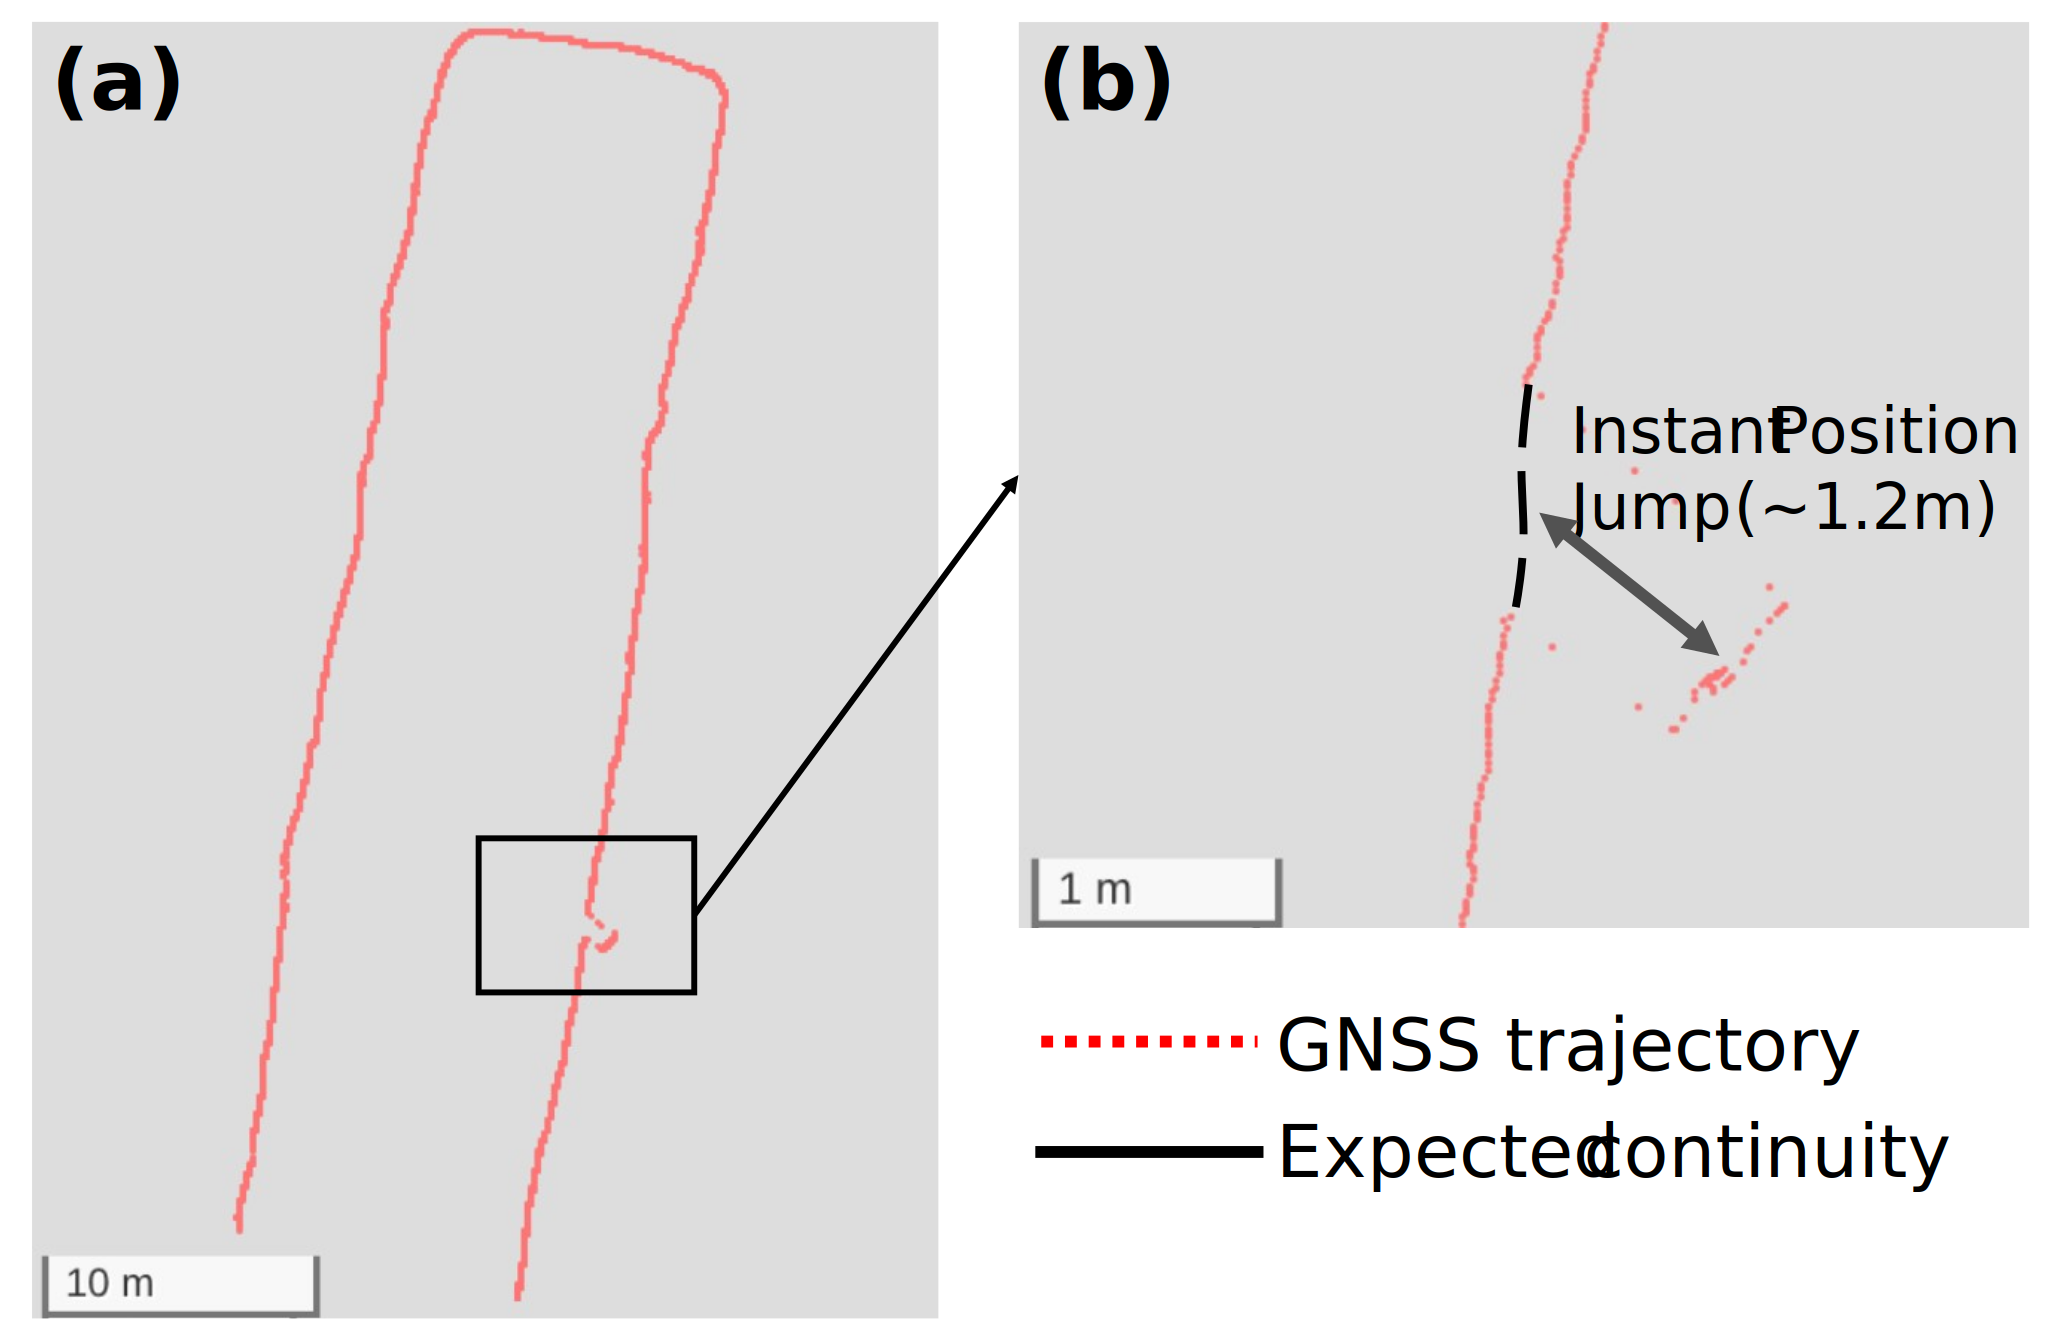
\includegraphics[width=\linewidth]{figures/3/10_23_2.png} 
  \caption{GNSS trajectory discontinuity observed on Oct. 23, 2025.
(a) Global trajectory with the anomalous segment highlighted. 
(b) Enlarged view showing an instantaneous position jump of approximately 1.2 m, 
where the raw GNSS trajectory deviates from the expected continuity.}
  \label{fig:gnss_jump_1023}
\end{figure}

\begin{figure}[tb]
  \centering
  \includegraphics[width=\linewidth]{figures/3/fix_timeseries_0_130.pdf}
  \caption{
  Time histories of the GNSS incremental displacement $|\Delta p_{\mathrm{gnss}}|$ and the covariance trace
  $\mathrm{trace}(\Sigma_{\mathrm{gnss}})$ for the 2025-10-23 dataset.
  Only the first 130~s are shown to focus on the interval around the detected trajectory discontinuity in
  Fig.~\ref{fig:gnss_jump_1023}.}
  \label{fig:gnss_fix_timeseries_1023}
\end{figure}


\begin{figure}[tb]
  \centering
  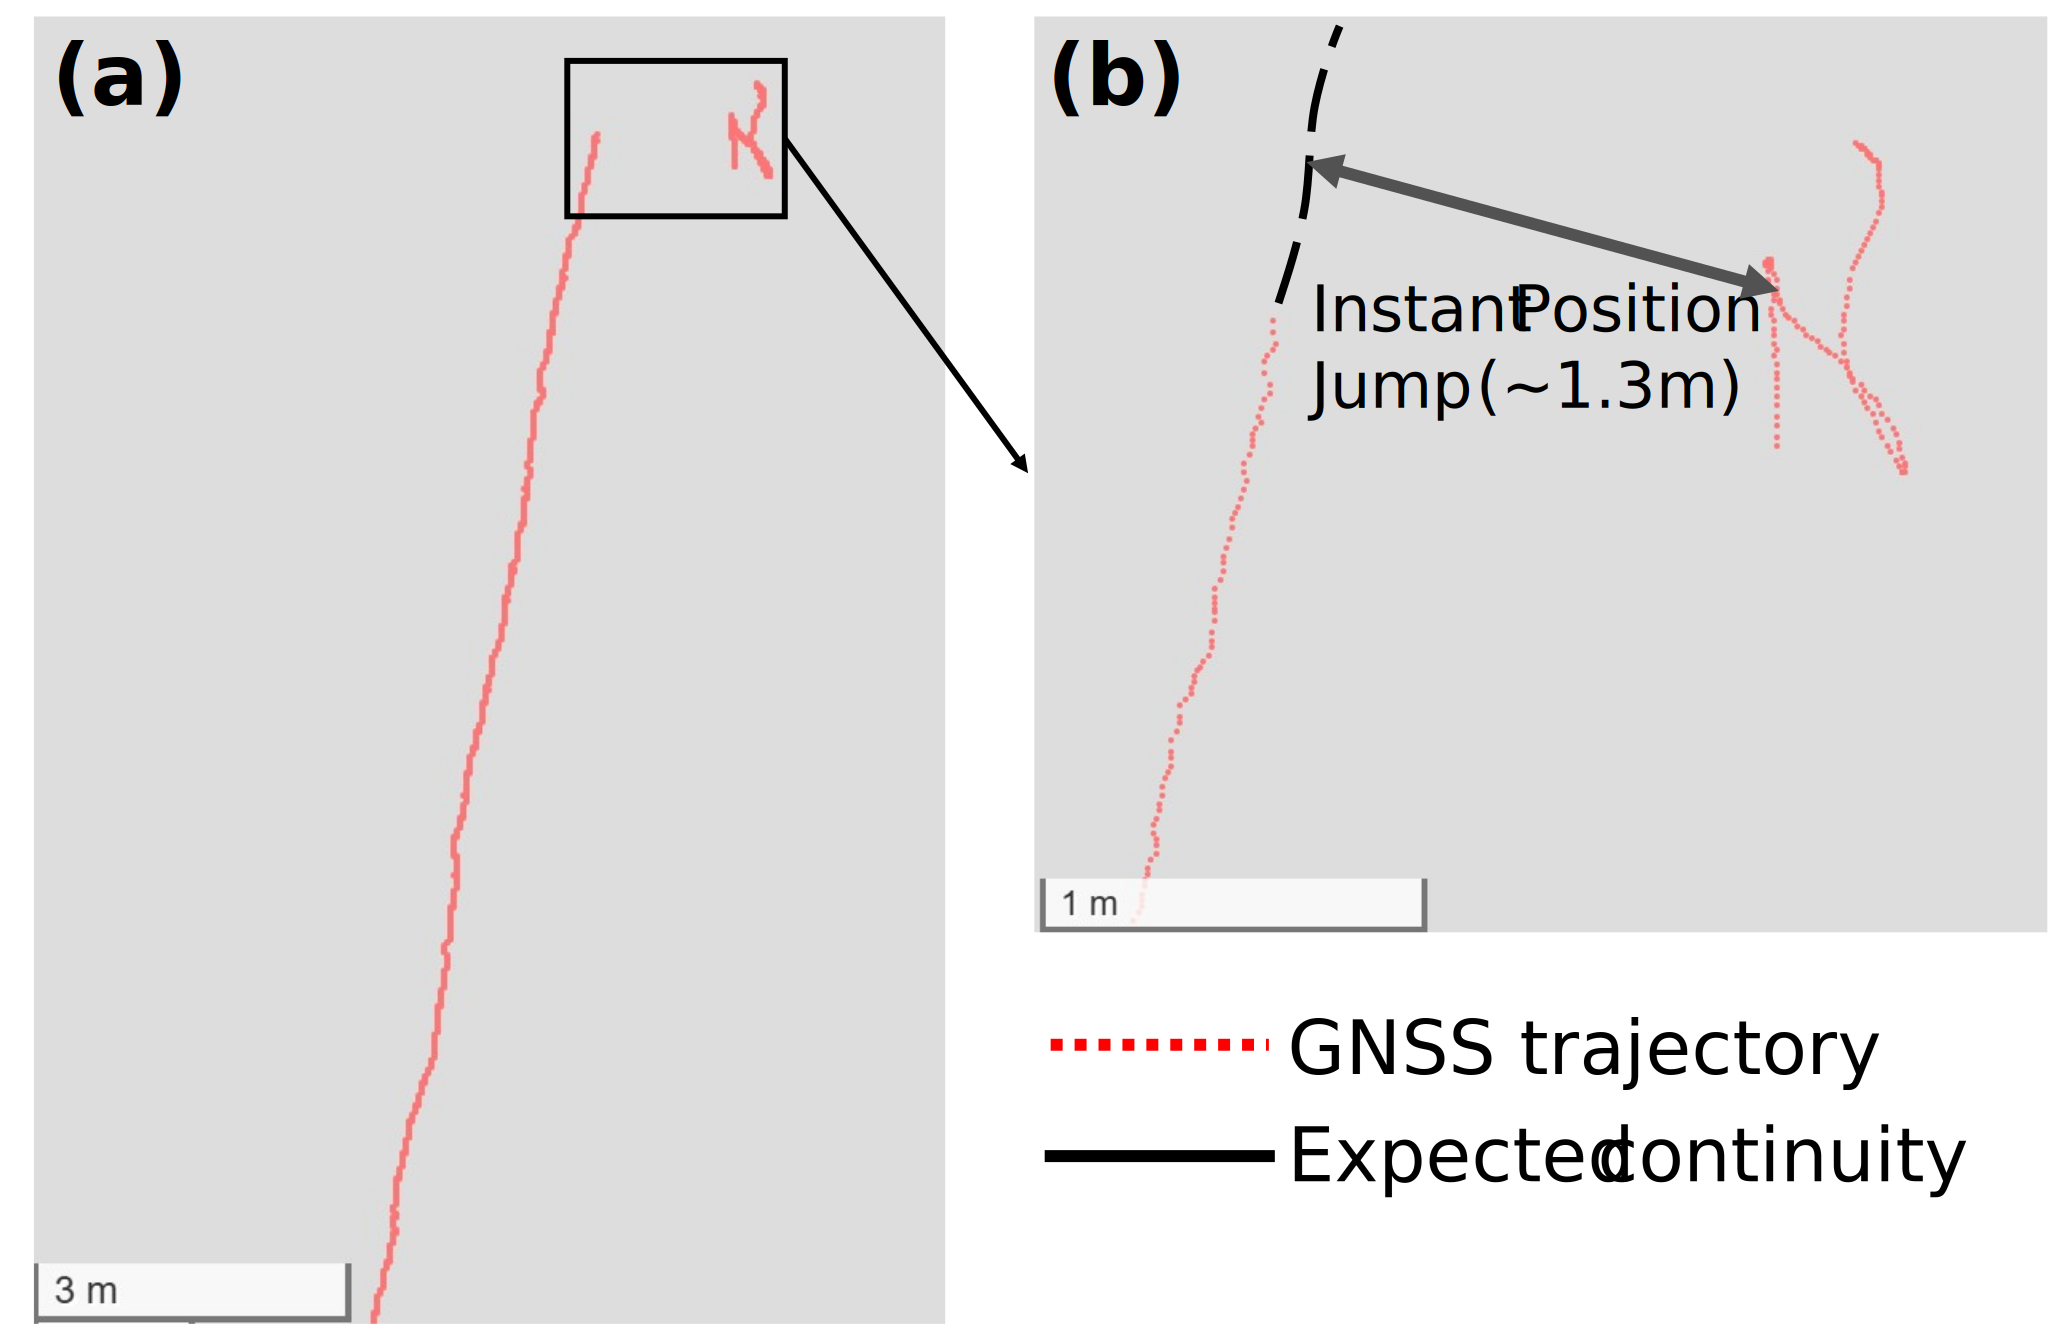
\includegraphics[width=\linewidth]{figures/3/10_20_2.png}
  \caption{GNSS trajectory discontinuity observed on Oct. 20, 2025.
  (a) Global trajectory overview. 
  (b) Enlarged view showing a similar instantaneous position jump of approximately 1.3 m, 
  indicating the reproducibility of the phenomenon.}
  \label{fig:gnss_jump_1020}
\end{figure}

\subsection{比較手法と設定}
\label{subsec:methods_compared}
本評価では以下の3つの手法を比較する.
いずれの手法においても,入力となるLiDARおよびIMUのデータは共通とし,
RTAB-Mapのパラメータ設定も統一した.
まず,GNSS情報を利用せず,FAST-LIO2によるオドメトリのみを用いてマッピングを行うLIO単独である.
次に,GNSSの品質を考慮せず,得られた観測値をそのままRTAB-Mapの位置制約として導入する単純統合である.
そして最後が,提案するGNSS品質監視モジュールによって観測の採否を判定し,信頼できるデータのみをRTAB-Mapへ入力する提案手法である.

\subsection{評価指標}
\label{subsec:metrics}
本実験を行う農業用ハウス環境では,
走行軌跡を高精度な計測器による真値の取得が困難である.
また,RTK-GNSS自体が不安定であるため,
GNSSを正解として使うこともできない.
そこで本研究では,地図や軌跡の整合性に着目して定性的な評価を行う.

評価の観点は以下の3点である.
第1に点群地図の重なりを確認する.同じ場所を何度も通ったときに,
壁面や柱等の構造物に矛盾した重なりが発生していないかを視認し,地図の歪みを評価する.
第2に軌跡の滑らかさを確認する.車両の運動学的制約に反する,
非連続な位置の跳躍の有無を確認する.
第3に復帰時の挙動を確認する.GNSSが不安定な状態から回復したときに,
誤った拘束が地図構造の破綻を引き起こさないかを確認する.
また,提案手法の動作確認として,システムがデータを遮断
したタイミングが適切かどうかも併せて確認する.

\subsection{走行軌跡の比較}
\label{subsec:traj_compare}

提案手法と従来手法(品質監視なし)の差を示すため,
RTAB-Mapが出力する\texttt{map}座標系の走行軌跡を比較した.
なお,両軌跡は走行開始直後の短時間区間を基準として位置・方位を整列し,
形状差が視覚的に比較できるようにした.

\begin{figure}[htbp]
    \centering
    \begin{minipage}[b]{0.48\textwidth}
        \centering
        \includegraphics[width=\textwidth]{figures/3/traj_global.png}
        \caption{Comparison of trajectories between the proposed method and the naive method.}
        \label{fig:traj_global}
    \end{minipage}
    \hfill
    \begin{minipage}[b]{0.48\textwidth}
        \centering
        \includegraphics[width=\textwidth]{figures/3/traj_zoom_A.png}
        \caption{Enlarged view around point A (NLOS-affected segment) in Fig.~\ref{fig:traj_global}.}
        \label{fig:traj_zoom_A}
    \end{minipage}
\end{figure}


Fig.~\ref{fig:traj_global}より,全体としては両手法で類似した軌跡が得られている一方で,
特定区間において従来手法の軌跡が局所的に逸脱していることが分かる.
Fig.~\ref{fig:traj_zoom_A}は,差が最も顕著であった区間Aの拡大図である.
AはGNSSのNLOS影響が疑われる区間であり,
従来手法では品質低下したGNSS観測が拘束として混入することで,
軌跡の逸脱が生じたと考えられる.
一方,提案手法ではGNSS観測を品質監視により遮断し,
同区間における推定の安定化を確認した.

\begin{figure}[tb]
  \centering
  \includegraphics[width=\linewidth]{figures/3/traj_error.png}
  \caption{Positional difference over time between the proposed and naive methods.}
  \label{fig:traj_error}
\end{figure}

なお,ハウス間の通路のように周囲構造が少ない区間では,
LiDAR点群が疎になりやすく,Fig.~\ref{fig:traj_global}のBに示すように,
LIOが縮退して不安定となる場合がある.
この現象はGNSSのNLOS影響とは別の要因で生じるため,
本研究ではAに示すNLOS影響が疑われる区間を主な比較対象として示した.


\subsection{評価結果と考察}
\label{subsec:real_world_results}


前節では,提案手法と従来手法(品質監視なし)の走行軌跡を比較し,
Fig.~\ref{fig:traj_global}~Fig.~\ref{fig:traj_error}では差が顕著に現れる区間を拡大して示す.
次に,点群地図の比較により,誤った拘束の混入が地図に与える影響を確認する.

2025年10月23日の走行データを用いた各手法の点群地図と推定軌跡の
比較をFig.~\ref{fig:map_comparison_4panel}に示す(白:点群地図,黄:推定軌跡).
単純統合では,地図全体を俯瞰すると後続の最適化によって整合しているように見える場合があるが,
異常発生の直後(Fig.~\ref{fig:map_comparison_4panel}(b))において,
局所的な地図のズレや歪みが観測された.これは,
誤ったGNSS制約が因子グラフに導入された影響であると考えられる.
これに対し,LIO単独ではGNSSを用いないため外れ値の影響は受けないものの,
長期的なドリフトを抑制するための絶対的な制約が得られないという課題がある
(Fig.~\ref{fig:map_comparison_4panel}(c)).
一方,提案手法では,異常が疑われる区間のGNSS観測を適切に遮断することで,
局所的な歪みが抑制されることを確認した(Fig.~\ref{fig:map_comparison_4panel}(d)).

\clearpage
\begin{figure}[tb]
  \centering

  % Row 1: Naive (overview + zoom-in)
  \begin{subfigure}[t]{0.49\linewidth}
    \centering
    \includegraphics[width=\linewidth,height=0.36\textheight,keepaspectratio]{figures/3/LIO_NLOS_FIX_all.png}
    \caption{Naive GNSS-LIO fusion, where the boxed region indicates the area around the observed anomaly.}
    \label{fig:naive_overview}
  \end{subfigure}
  \hfill
  \begin{subfigure}[t]{0.49\linewidth}
    \centering
    \includegraphics[width=\linewidth,height=0.36\textheight,keepaspectratio]{figures/3/LIO_NLOS_FIX_part.png}
    \caption{Enlarged view of the boxed region in (a)}
    \label{fig:naive_zoom}
  \end{subfigure}

  \vspace{2mm}

  % Row 2: LIO単独 vs Proposed
  \begin{subfigure}[t]{0.49\linewidth}
    \centering
    \includegraphics[width=\linewidth,height=0.36\textheight,keepaspectratio]{figures/3/Only_LIO.png}
    \caption{LIO-only mapping without GNSS constraints.}
    \label{fig:lio_only}
  \end{subfigure}
  \hfill
  \begin{subfigure}[t]{0.49\linewidth}
    \centering
    \includegraphics[width=\linewidth,height=0.36\textheight,keepaspectratio]{figures/3/LIO+proposed.png}
    \caption{Mapping result with the proposed method.}
    \label{fig:proposed}
  \end{subfigure}

  \caption{
  Mapping results for the 2025-10-23 dataset (white: point cloud map, yellow: estimated trajectory).
  }
  \label{fig:map_comparison_4panel}
\end{figure}
\clearpage

また,NLOSの影響をより明確に示すため,
単純統合における異常発生直後の局所的な挙動をFig.~\ref{fig:map_comparison_4panel}(b)に示す.
本走行データでは,異常の発生直後に地図の歪みが生じたが,
その後の整合的な観測やループ閉じ込みによって,
全体的な誤差が解消される挙動も確認された.
しかし,このような回復が常に保証されるものではなく,
異常の規模や発生タイミングによっては,地図の整合性が著しく損なわれ,
回復不能となる恐れがある.したがって,異常の疑われる観測値を事前に選別し,
最適化から排除することが重要である.

提案手法による異常検知のプロセスを確認するため,
2025年10月23日のデータにおけるNISと判定結果の時系列を 
Fig.~\ref{fig:timeline_1023}に示す.図中の破線は閾値$\gamma_{\mathrm{pass}}$を,
上部のバーはデータの採用/遮断を表す.異常が発生した区間ではNISが急増しており,
GNSS観測が適切に排除されていることが分かる.
また,NISが閾値以下であっても,可用性判定や復帰時の遮断される場合がある.
これは,誤った拘束が因子グラフへ混入することを確実に防ぐための判定によるものである.


\begin{figure}[t]
  \centering
  \includegraphics[width=\linewidth]{figures/3/timeline_1023.pdf}
  \caption{Time history of the median NIS and the acceptance decision for the 2025-10-23 dataset.
The dashed line indicates the threshold $\gamma_{\text{pass}}$, and the color bar shows the PASS/FAIL decision.}
  \label{fig:timeline_1023}
\end{figure}

本評価により,実環境で発生するGNSSの測位異常に対し,
品質監視によって地図の整合性を維持できることを確認した.
一方で,本実験環境では異常の発生頻度が限定的であったため,
統計的な信頼性を高めるには追加の長時間のデータ収集が必要である.
今後は,複数のデータセットを用いて,
提案手法の再現性を検証することが課題である.

\end{document}